\documentclass[]{rAMF2e}
%\usepackage[square]{natbib}
%\usepackage{authblk}
\usepackage{listings}
\usepackage[center]{caption}
\usepackage{hyperref}


\begin{document}
\doi{}
\issn{}  \issnp{}
\jvol{00} \jnum{00} \jyear{2013} %\jmonth{January--March}
\def\jobtag{}
\publisher{Unpublished}
\jname{}

\markboth{Fabien {Le Floc'h} and Gary Kennedy}{Draft}

\title{Explicit SABR Calibration through Simple Expansions}
\author{Fabien {Le Floc'h}$^\star$\thanks{{\em{Correspondence Address}}: Calypso Technology, 106 rue de La Bo\'{e}tie, 75008 Paris. Email: \texttt{fabien\_lefloch@calypso.com} \vspace{6pt}} and Gary Kennedy$^\dag$}
\affil{$^\star$Calypso Technology, 106 rue de La Bo\'{e}tie, 75008 Paris\\$^\dag$Clarus Financial Technology, London}
%
\date{\today}
\received{v1.0 released June 2014}

\maketitle
\newcommand{\sgn}{\mathop{\mathrm{sgn}}}
\begin{abstract}
The SABR stochastic volatility model is a very popular interpolator of implied volatilities, with a given dynamic. This paper presents a simple and very fast method to calibrate the SABR model to given market volatilities, that is to imply the SABR parameters from a given market smile.
\begin{keywords}stochastic volatility, SABR, calibration, implied volatility, finance\end{keywords}
\end{abstract}

\section{Introduction}
The SABR stochastic volatility model \citep{hagan2002managing} enjoys a high popularity as interpolator of implied volatilities, because, in practice, it fits rather well market implied volatility smiles for interest rate derivatives, fx derivatives and equity derivatives with a few parameters $\alpha, \rho, \nu$, and the dynamic of it can be easily controlled through its $\beta$ parameter, usually defined from historical series analysis for the relevant market.

There are however known shortcomings: it is not arbitrage free as the probability density can become negative for low strikes and long maturities. Many authors have proposed various improvements to the original formula \citep{obloj2008fine, johnson2009arbitrage, paulot2009asymptotic, benaim2008arbitrage}. More recently the focus has been on finite difference techniques to guarantee the arbitrage-free property \citep{andreasen2011zabr, hagan2013arbitrage,lefloch2014fdmsabr} in a shifted SABR framework, to allow for negative rates. 

In practice, the adjustments to the original formula do not matter much in order to find a good initial guess for the calibration procedure. Once a good initial guess is found, a fast local minimizer like Levenberg-Marquardt can be used to calibrate the specific SABR implementation. 

A first calibration method was described in \citep{west2005calibration}, fitting $\alpha$ exactly to the at-the-money implied volatility, and reducing the problem to a two-dimensional minimization in $(\rho,\nu)$. The Nelder-Mead method is proposed as the minimizer. However, it still requires an initial guess, and can sometimes be unstable, especially with constraints \citep{lefloch2014nelder}. A numerical method to find an initial guess that fits the at-the-money volatility exactly and the at-the-money skew is proposed in \citep{gauthier2009fitting}. It requires the numerical solution of a two-dimensional non linear system of equations.

In contrast, the method proposed here is simple and explicit; a system of equations to fit the at-the-money volatility, skew, and curvature is solved analytically. A similar approach was applied to the Heston model in \citep{forde2012small} with the difference that, in their case, the Heston parameters describe a full volatility surface and the initial guess procedure relies on two expiries plus the short time at-the-money volatility to solve the 5 Heston parameters exactly. In the SABR case, there is just one expiry to consider and 3 parameters to fit. We will first present our method for the lognormal formula as well as for the normal formula, and then show its accuracy in calibrating real world smiles on the arbitrage-free model from \citet{hagan2013arbitrage} compared to a global optimization via differential evolution.


\section{SABR normal and lognormal formulas}

\subsection{The SABR model}
In the shifted SABR model, the asset forward follows the following stochastic equation:
\begin{align}
dF &= V (F+b)^\beta dW_1\\
dV &= \nu V dW_2
\end{align}
with $W_1, W_2$ Brownian motions correlated with correlation $\rho$,
and $F(0) = f$, $V(0) = \alpha$.
$\nu$ represents the volatility of volatility, $b$ is a displacement allowing for negative rates ($b=0$ for the classic SABR model).

\subsection{Normal formula}
Given the low rates environment we currently experience, it is now common practice to quote swaptions in terms of normal volatility (bpvol). Taking into account the remarks from \citet{obloj2008fine} for the case of the lognormal formula to ensure consistency when $\beta \to 1$, the expansion of the normal volatility adapted from \citet{hagan2002managing} for the shifted SABR model is:

for $f \neq K$ and $\beta \in [0,1]$
\begin{align}
\label{eqn:normal_sabr}
\sigma_N(K) &= \frac{f-K}{x(K)}\left[1+\left(g(K)+\frac{1}{4}\rho\nu\alpha\beta(f+b)^{\frac{\beta-1}{2}}(K+b)^{\frac{\beta-1}{2}}+\frac{1}{24}(2-3\rho^2)\nu^2\right)T\right]
\end{align}
with 
\begin{align*}
g(K) &= \frac{1}{24} (\beta^2-2\beta) (f+b)^{\beta-1} (K+b)^{\beta-1} \alpha^2\\
\zeta(K) &= \frac{\nu}{\alpha (1-\beta)} \left( (f+b)^{1-\beta} - (K+b)^{1-\beta} \right)\\
x(K) &= \frac{1}{\nu}\log\left(\frac{\sqrt{1-2\rho\zeta(K)+\zeta^2(K)}-\rho+\zeta(K)}{1-\rho} \right)
\end{align*}

When $f=K$, 
\begin{align}
\sigma_N(f) &= \alpha (f+b)^\beta \left[1+\left(g(f)+\frac{1}{4}\rho\nu\alpha\beta(f+b)^{\beta-1}+\frac{1}{24}(2-3\rho^2)\nu^2\right)T\right]
\end{align}

When $\beta = 1$,
\begin{align*}
g(K) = -\frac{1}{24}\alpha^2 &\texttt{ , } \zeta(K) = \frac{\nu}{\alpha} \log\left(\frac{f+b}{K+b}\right)
\end{align*}

When $\beta = 0$,
\begin{align*}
g(K) = 0 &\texttt{ , }\zeta(K) = \frac{\nu}{\alpha} \left(f-K\right)
\end{align*}
%recap of SABR Hagan 2002 formula and obloj
\subsection{Lognormal formula}
The lognormal formula is very similar to the normal formula, $f-K$ becomes $\log(\frac{f}{K})$ and $g$ includes a small adjustment:

for $f \neq K$ and $\beta \in [0,1]$,
\begin{align}
\sigma_B(K) &= \frac{1}{x(K)}\log\left(\frac{f+b}{K+b}\right)\left[1+\left(g(K)+\frac{1}{4}\rho\nu\alpha\beta(f+b)^{\frac{\beta-1}{2}}(K+b)^{\frac{\beta-1}{2}}+\frac{1}{24}(2-3\rho^2)\nu^2\right)T\right]
\end{align}
with 
\begin{align*}
g(K) &= \frac{1}{24} (\beta-1)^2 (f+b)^{\beta-1} (K+b)^{\beta-1} \alpha^2\\
\zeta(K) &= \frac{\nu}{\alpha (1-\beta)} \left( (f+b)^{1-\beta} - (K+b)^{1-\beta} \right)\\
x(K) &= \frac{1}{\nu}\log\left(\frac{\sqrt{1-2\rho\zeta(K)+\zeta^2(K)}-\rho+\zeta(K)}{1-\rho} \right)
\end{align*}

When $f=K$, 
\begin{align}
\sigma_B(f) &= \alpha (f+b)^{\beta-1} \left[1+\left(g(f)+\frac{1}{4}\rho\nu\alpha\beta(f+b)^{\beta-1}+\frac{1}{24}(2-3\rho^2)\nu^2\right)T\right]
\end{align}

When $\beta = 1$,
\begin{align*}
g(K) = 0 &\texttt{ , } \zeta(K) = \frac{\nu}{\alpha} \log\left(\frac{f+b}{K+b}\right)
\end{align*}

When $\beta = 0$,
\begin{align*}
g(K) = \frac{1}{24(f+b)(K+b)}\alpha^2 &\texttt{ , }\zeta(K) = \frac{\nu}{\alpha} \left(f-K\right)
\end{align*}
It is important not to forget that Hagan derived the lognormal formula as an approximation of the normal formula \citep{hagan2002managing}: it won't be accurate or realistic at all in cases where the implied volatility is very high (see Table \ref{tbl:lognormal_high_alpha}). This is not so realistic for market implied volatilities, but it can have an influence in the global minimization procedure, as global minimizers like differential evolution will try out extreme values.

Of course, in order to obtain a lognormal volatility, it is also possible to solve, with high accuracy, for the Black implied volatility of a given normal volatility: we can firstly compute corresponding Bachelier option price with a fast evaluation method \citep{lefloch2014bpvol} and secondly use a robust and accurate Black implied volatility solver \citep{jackel2013let, li2011adaptive}.

\begin{table}[h]
\begin{center}
\caption{\label{tbl:lognormal_high_alpha}Black volatility obtained from the direct lognormal approximation compared the one solved from the normal approximation using $\alpha=3.24,\beta=1.0,\rho=-0.998, \nu=1.69, f=2014, K=f, T=0.48$.}
\begin{tabular}{|c|c|c|}
\hline
Formula & Black volatility & Option price \\ 
\hline
Lognormal & 0.9325 & 510.19 \\
Normal & 0.2526 & 140.41 \\
\hline
\end{tabular}
\end{center}
\end{table}
%bachelier price can be infinite when bachelier vol high, while blackscholes is 0
%solving can break down in those cases.
For performance reasons, we prefer to rely on the normal formula if the calibration is for bpvols and the lognormal formula if the calibration is for Black volatilities.

%\subsection{Latest Hagan normal formula}
%mention of latest Hagan formula 2014

\section{Explicit initial guess}
\subsection{Lognormal volatility}
The idea is to find $\alpha, \rho, \nu$ that matches the at-the-money implied volatility $\sigma_0$, skew $\sigma_0'$ and curvature $\sigma_0''$. A direct application of Hagan formula would lead to a system of trivariate polynomials of degrees 3 and 4, which would then require a numerical method. Instead, we rely a simple lower order expansion of the lognormal formula in the variable $z=\log\left(\frac{K+b}{f+b}\right)$ around $z=0$ that still captures the smile around the at-the-money level accurately:

\begin{align}
\sigma_B(z) &= \alpha (f+b)^{\beta-1} + \frac{1}{2}\left(\rho \nu - (1-\beta)\alpha (f+b)^{\beta-1}\right)z \nonumber\\
&+ \frac{1}{12\alpha (f+b)^{\beta-1}}\left((1-\beta)^2(\alpha (f+b)^{\beta-1})^2 + \nu^2(2-3\rho^2)\right)z^2
\end{align}

This is the same expansion used in \citep[equation (3.1a)]{hagan2002managing} to explain the phenomenology and dynamic of the SABR model. It can also be found from the expansion of \citep{lorig2014implied} by using the order-0 expansion for the at-the-money implied volatility, the order-1 expansion for the at-the-money skew, and the order-2 for the at-the-money curvature and ignore terms quadratic in time to expiry $T^2$. Or more simply it can be rederived from a Taylor expansion, neglecting higher order terms as in Appendix \ref{apx:normal_expansion}. We have then:
% expansions obtained with the formula from \citep{lorig2014implied}. Applied to the shifted SABR model, their second order expansion of the implied volatility $v$ is $v = v_0 + v_1 + v_2$ where 
%lorig formula for order 2 %
%\begin{align*}
%v_0 &= \alpha (f+b)^{\beta-1}\\
%v_1 &= \frac{1}{2}(\beta-1) z v_0 + \frac{1}{2}z\rho\nu+ \frac{1}{4}T\nu v_0(\rho v_0 - \nu)\\
%v_2 &= \frac{1}{96}(\beta-1)^2 v_0 \left(8z^2+T v_0 (4-T v_0^2)\right)\\
%&- \frac{1}{48}T(\beta-1)\nu v_0 \left(6z\nu+2(6-5z)\rho v_0 + T\rho v_0^3\right)\\
%&+ \frac{1}{96}T\nu^2 v_0 \left(32 + 5T\nu^2 - 12 \rho^2 + 2T v_0((6\rho^2-2)v_0-7\nu\rho) \right)\\
%&- \frac{1}{24}T\nu^2\rho (\nu-3\rho v_0) z+\frac{\nu^2(2-3\rho^2)}{12}z^2
%\end{align*}
% We use the order-0 expansion for the at-the-money implied volatility, the order-1 expansion for the at-the-money skew, and the order-2 for the at-the-money curvature and ignore terms quadratic in time to expiry $T^2$. Note that the derivatives are expressed in log-moneyness towards the variable $z=\log(\frac{K+b}{f+b})$ where $K$ is the strike and $f$ is the forward. We have then:
\begin{align}
\begin{cases}
\sigma_0 &= \alpha(f+b)^{\beta-1}\\
\sigma_0' &= \frac{1}{2}\left(\rho \nu - (1-\beta)\sigma_0\right)\\
\sigma_0'' &= \frac{1}{3\sigma_0}\nu^2+\frac{1}{6\sigma_0}\left((1-\beta)^2\sigma_0^2 - 3\rho^2\nu^2\right)
\end{cases}
\end{align} 
Note that the derivatives are expressed on log-moneyness, $z$.

This system can be exactly solved to give a first guess $\alpha_0, \rho_0,\nu_0$:
\begin{align}
  \begin{cases}
\alpha_0 &=  \sigma_0 (f+b)^{1-\beta}\\
\nu_0^2 &= 3\sigma_0\sigma_0''-\frac{1}{2}(1-\beta)^2\sigma_0^2+\frac{3}{2}\left(2\sigma_0'+(1-\beta)\sigma_0\right)^2 \\
\rho_0 &= \frac{1}{\nu_0}\left(2\sigma_0'+(1-\beta)\sigma_0\right) 
\end{cases} 
\end{align}
We make sure to constrain $\nu_0$ to be strictly positive (for example by flooring it to $10^{-4}$) , and $\rho_0$ to be in [-1,1]. We then refine this first guess by solving exactly for the at-the-money volatility with the given $\rho_0$ and $\nu_0$. $\alpha_1$ is the root of the following third order polynomial:
\begin{align}
\frac{(1-\beta)^2 T}{24 (f+b)^{2-2\beta}}\alpha^3+ \frac{\rho\beta\nu T}{4(f+b)^{1-\beta}}\alpha^2 + \left(1+\frac{2-3\rho^2}{24}\nu^2 T\right)\alpha - \sigma_0 (f+b)^{1-\beta} &= 0
\end{align}
This is the same polynomial used by \citet{west2005calibration} to reduce the dimension of the calibration problem: $\alpha_1$ is chosen as the smallest positive root. In theory, choosing $\alpha_1$ closest to the previously calibrated $\alpha$ (either from the previous expiry, or from a previous day) could be better. In practice, it turns out to always be the smallest positive root. 
Our initial guess is then $(\alpha_1, \rho_0, \nu_0)$.
%We then compute $\nu_1, \rho_1$ based on this new $\alpha_1$.
%\begin{align}
%\sigma_1 &=  \alpha_1 (f+b)^{\beta-1}\\
%\nu_1^2 &= 3\sigma_1\sigma_0''-\frac{1}{2}(1-\beta)^2\sigma_1^2+\frac{3}{2}\left(2\sigma_0'+(1-\beta)\sigma_1\right)^2 \\
%\rho_1 &= \frac{1}{\nu_1}\left(2\sigma_0'+(1-\beta)\sigma_1\right)          
%\end{align}
\subsection{Normal volatility}
When the input volatilities are normal (bpvol), we can just convert them to equivalent lognormal volatilities and apply the same method as in the previous section to find the initial guess. In our case, because the initial guess method depends mostly on volatilities closest to the money, we can also rely on another simple expansion based on the work of \citep{lorig2014implied}:
\begin{align}
\sigma_B &= v_0 - \frac{1}{2}v_0 z + \frac{1}{96}v_0(8z^2+T v_0^2 (4-T v_0^2)) \nonumber \\
         &+ \frac{1}{192}T z v_0^3 (-12+5T v_0^2)
\end{align}
with $v_0 = \frac{\sigma_N}{f}$ and $z=\log(\frac{K}{f})$, where the last term is of order-3.

Instead, we prefer to work directly with normal volatility and derive a simple expansion of the normal formula in $z=\log\left(\frac{K+b}{f+b}\right)$ around $z=0$ (see Appendix \ref{apx:normal_expansion});

\begin{align}
\sigma_N(z) &= \alpha (f+b)^\beta + \frac{1}{2}\left(\rho \nu (f+b)+\beta \alpha (f+b)^\beta \right)z\nonumber\\
&+ \left[\frac{1}{12\alpha (f+b)^{\beta-2}}(2\nu^2-3\rho^2 \nu^2)+\frac{1}{4} \rho \nu (f+b)+\frac{1}{12}(\beta^2+\beta)\alpha (f+b)^\beta \right]z^2
\end{align}

Let $\sigma_0, \sigma_0', \sigma_0''$ be respectively the normal volatility, the slope and the curvature at the money expressed in log-moneyness $z$. We have:

\begin{align}
\begin{cases}
\sigma_0 &= \alpha (f+b)^{\beta}\\
\sigma_0' &= \frac{1}{2}\rho \nu (f+b) + \frac{1}{2} \beta \sigma_0\\
\sigma_0'' &= \frac{(f+b)^2}{6\sigma_0}(2\nu^2 - 3\rho^2\nu^2)+\frac{1}{2} \rho \nu (f+b)+\frac{1}{6}(\beta^2+\beta)\sigma_0
\end{cases}
\end{align}
This system can be exactly solved to give a first guess $\alpha_0, \rho_0,\nu_0$:
\begin{align}
  \begin{cases}
\alpha_0 &=  \sigma_0 (f+b)^{-\beta}\\
\nu_0^2 &= \frac{1}{(f+b)^2}\left[ 3\sigma_0\sigma_0''-\frac{1}{2}(\beta^2+\beta)\sigma_0^2-3\sigma_0(\sigma_0'-\frac{1}{2}\beta\sigma_0) +\frac{3}{2}\left(2\sigma_0'-\beta\sigma_0\right)^2\right] \\
\rho_0 &= \frac{1}{\nu_0 (f+b)}\left(2\sigma_0'-\beta\sigma_0\right) 
\end{cases} 
\end{align}
As for the lognormal volatility guess, we refine this first guess by solving exactly for the at-the-money volatility with the given 
$\rho_0$ and $\nu_0$. Then $\alpha_1$ is a root of the following third order polynomial:
\begin{align}
\frac{(\beta^2-2\beta) T}{24 (f+b)^{2-2\beta}}\alpha^3+ \frac{\rho\beta\nu T}{4(f+b)^{1-\beta}}\alpha^2 + \left(1+\frac{2-3\rho^2}{24}\nu^2 T\right)\alpha - \sigma_0 (f+b)^{-\beta} &= 0
\end{align}
Note that this polynomial is slightly different from the lognormal volatility polynomial. Again we take the $\alpha_1$ to be the smallest positive root.
 
  
%\subsubsection{Expansion of normal volatility at the money}
%A normal volatility $\sigma_N$ can be converted almost exactly to a lognormal volatility $\sigma_B$ by first pricing an out of the money option with the Bachelier formula, and inverting the price to find the lognormal volatility with an accurate solver \citep{jackel2013let}. 
%
\subsection{How to find the at-the-money volatility, slope and curvature?}
The simplest is to fit a parabola to the three closest points around the forward with coordinates $(z_{-1}, \hat{\sigma}_{-1}), (z_0,\hat{\sigma}_0), (z_{1},\hat{\sigma}_1)$. This is equivalent to a 3 points finite difference on a non uniform grid. We then have:
\begin{align}
\sigma_0 &= z_0 z_1 w_{-1} \hat{\sigma}_{-1} + z_{-1} z_1 w_{0} \hat{\sigma}_{0} +  z_{-1} z_0w_{1} \hat{\sigma}_{1}\\
\sigma_0' &= -(z_0 + z_1) w_{-1} \hat{\sigma}_{-1} - (z_{-1}+ z_1) w_{0} \hat{\sigma}_{0} -  (z_{-1}+ z_0)w_{1} \hat{\sigma}_{1}\\
\sigma_0'' &= 2 w_{-1} \hat{\sigma}_{-1} +2 w_{0} \hat{\sigma}_{0} + 2w_{1} \hat{\sigma}_{1}
\end{align}
with 
\begin{align}
w_{-1} &= \frac{1}{(z_{-1}-z_{0})(z_{-1}-z_{1})}\\
w_{0} &= \frac{1}{(z_{0}-z_{-1})(z_{0}-z_{1})}\\
w_{1} &= \frac{1}{(z_{1}-z_{-1})(z_{1}-z_{0})}
\end{align}
In our experience, using higher order approximations like a 5 points finite difference (equivalent to a quartic on 5 points), or a cubic spline does not lead to any visible improvement in accuracy on our problem.
 
When the input data is noisy, it can be useful to resort to a best fit parabola around the five or seven closest points from the forward, which can be reduced to solving simple linear system (Appendix \ref{apx:parabola}). When the volatility at the forward is already present in the input data, we can also make sure that the parabola passes exactly through it. We have noticed that including further away points in the estimation of the at-the-money curvature could be particularly important when the curvature is relatively small, for example for long-term options quotes (10 to 20 years) with a bit of noise. In some extreme situations, the three points curvature can be slightly negative and not allow for a good initial guess, as it can not represent such curvatures, while the seven points curvature will be accurate enough.

Another approach would be to repeat the initial guess procedure with a parabola on different sets of three points further away from the forward and select the guess corresponding to the best overall fit.

In our numerical tests we will select the guess that gives the minimum mean square error in volatilities between the two guesses stemming from the 3-points parabola and the 7-points parabola.
\section{Almost exact inversion of SABR smiles}
We use the SABR parameters found by calibration of the lognormal SABR model on the S\&P500 options in December 2008 as starting point (Table \ref{tbl:smart_initialguess_sabr_input}). From those we regenerate a discrete set of implied volatilities for 12 strikes and 11 expiries using the lognormal SABR formula with $\beta = 1$. And finally we apply the explicit initial guess procedure to each expiry.

%add guess alpha1 parameters in following table
%      REFERENCE     EXPLICIT GUESS
% exp  a  r  n       a    r   n

\begin{table}[h]
\begin{center}
\caption{\label{tbl:smart_initialguess_sabr_input}Reference SABR parameters with $f=2016$ and explicit guess}
\begin{tabular}{c|c c c|c c c c}
\hline
Expiry & \multicolumn{3}{|c|}{Reference parameters} & \multicolumn{4}{|c}{Explicit guess}\\
years & $\alpha$ & $\rho$ & $\nu$ & $\alpha$ & $\rho$ & $\nu$ & vol RMSE \\ 
\hline
0.058&	0.271&	-0.345&	1.010 & 0.271 & -0.343 & 1.008 & 2.64e-04 \\
0.153&	0.256&	-0.321&	0.933 & 0.256 & -0.319 & 0.934 & 1.36e-04\\
0.230&	0.256&	-0.346&	0.820 & 0.256 & -0.344 & 0.822 & 1.13e-04\\
0.479&	0.255&	-0.370&	0.629 & 0.255 & -0.369 & 0.631 & 8.25e-05\\
0.729&	0.257&	-0.403&	0.528 & 0.257 & -0.402 & 0.528 & 2.30e-05\\
1.227&	0.260&	-0.429&	0.448 & 0.260 & -0.429 & 0.447 & 6.15e-05\\
1.726&	0.261&	-0.440&	0.392 & 0.261 & -0.440 & 0.390 & 1.17e-04\\
2.244&	0.262&	-0.445&	0.355 & 0.262 & -0.445 & 0.352 & 1.59e-04\\
2.742&	0.262&	-0.445&	0.329 & 0.262 & -0.445 & 0.326 & 1.85e-04\\
3.241&	0.262&	-0.447&	0.310 & 0.262 & -0.447 & 0.306 & 2.13e-04\\
4.239&	0.263&	-0.452&	0.284 & 0.263 & -0.452 & 0.279 & 2.67e-04\\
\hline
\end{tabular}
\end{center}
\end{table}

The root mean square error in implied volatilities of the fit is always lower than $3\cdot 10^{-4}$. $\rho, \nu$ are recovered with an accuracy higher than $5\cdot 10^{-3}$ and $\alpha$ is recovered with and accuracy higher than $10^{-4}$, independently of the expiry (see Table \ref{tbl:smart_initialguess_sabr_input}). The refinement $\alpha_1$ allows to gain one order of magnitude in accuracy over $\alpha_0$, we display the various stages of the initial guess procedure on the slice of expiry 0.479 on Figure \ref{fig:smart_initialguess_sabr_input}.
\begin{figure}[htbp]
  \caption{\label{fig:smart_initialguess_sabr_input}The various stages of the initial guess method for the slice of expiry 0.479 year}
\begin{center}
 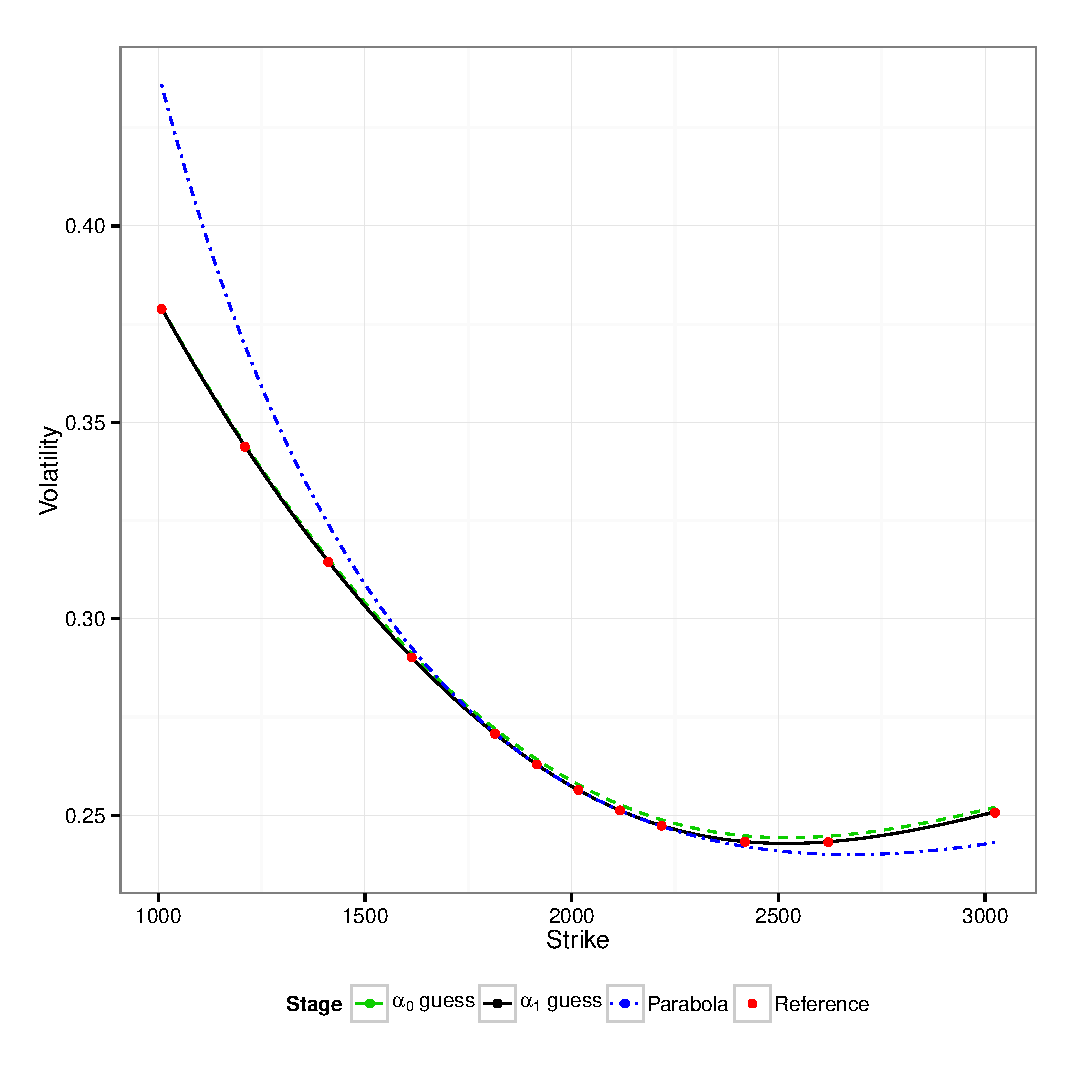
\includegraphics[width=16cm]{explicit_fit_sabr_0479_beta1.eps}
\end{center}
\end{figure}

\section{Real world smiles}
\subsection{Calibration on the analytic formula}
\subsubsection{Equity option smiles}
To calibrate SABR to equity implied volatility surfaces from December 2012, we minimize the weighted root mean square error in implied volatilities with the Levenberg-Marquardt method \citep{levenberg1944method,marquardt1963algorithm}, placing more weight to volatilities around ATM +/- 20\%. We compare the results obtained using either our explicit method as initial guess, or alternatively a guess found by running the differential evolution algorithm \citep{storn1997differential} with a population size 20 on 1000 generations. The resulting mean square error is displayed in Figure \ref{fig:explicit_de_equity_error}.

\begin{figure}[!h]
  \caption{\label{fig:explicit_de_equity_error}Root mean square error of calibration per expiry on various equity surfaces}
\begin{center}
 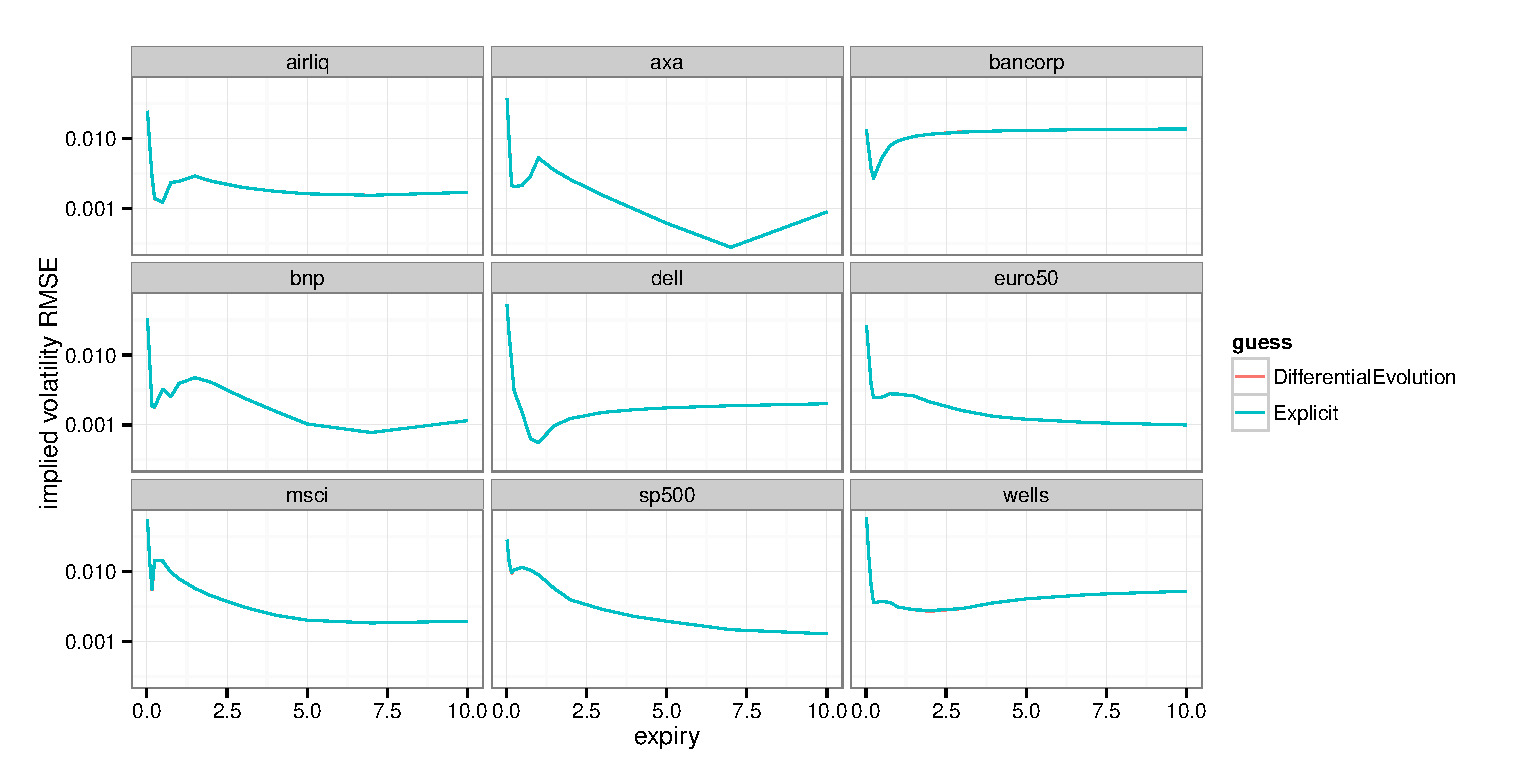
\includegraphics[width=16cm]{explicit_de_equity_error.eps}
\end{center}
\end{figure}

The minimization on the explicit guess leads to a mean square error in implied volatilities nearly indistinguishable from a minimization on the differential evolution guess. It is interesting however to look at the calibrated parameters values: the calibrated $\alpha$ shows some strong variations with the guess found by differential evolution, while it is relatively smooth with our explicit initial guess (Figure  \ref{fig:explicit_de_equity_alpha}). $\rho$ and $\nu$ behave similarly. We will take a closer look at why this happens in the next section.
\begin{figure}[!h]
  \caption{\label{fig:explicit_de_equity_alpha}Calibrated $\alpha$ on various equity surfaces}
\begin{center}
 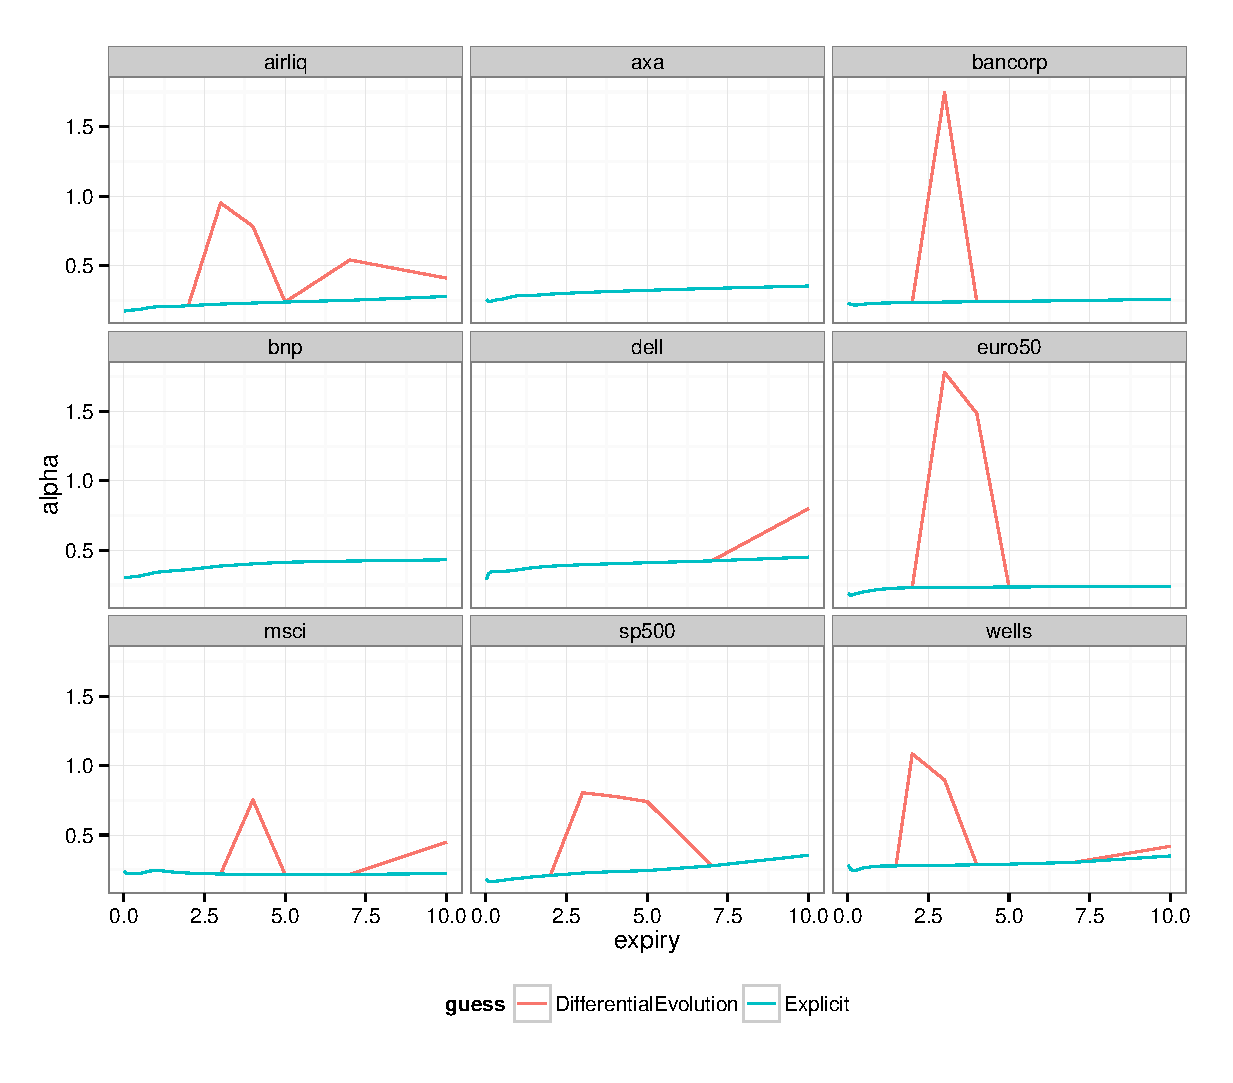
\includegraphics[width=16cm]{explicit_de_equity_alpha.eps}
\end{center}
\end{figure}


\subsubsection{Two SABRs for the same smile}
Figure \ref{fig:two_sabr_1_smile} illustrates how two different sets of SABR parameters can lead to an equally good fit. We just picked the S\&P 500 options expiring in 4 years used in the previous section. The root mean square error is  0.00219269910750194 for the SABR parameters with lower $\alpha$ while the one for the higher $\alpha$ is 0.002192699107502103, that is the lower $\alpha$ fits better by only $10^{-16}$.

\begin{figure}[htbp]
  \caption{\label{fig:two_sabr_1_smile}Smiles corresponding to $\alpha= 0.237, \rho= -0.735, \nu= 0.398$ and $\alpha= 0.850, \rho= -0.742, \nu= 1.335$ with $\beta=1, f=1426.19, T=4$}
\begin{center}
 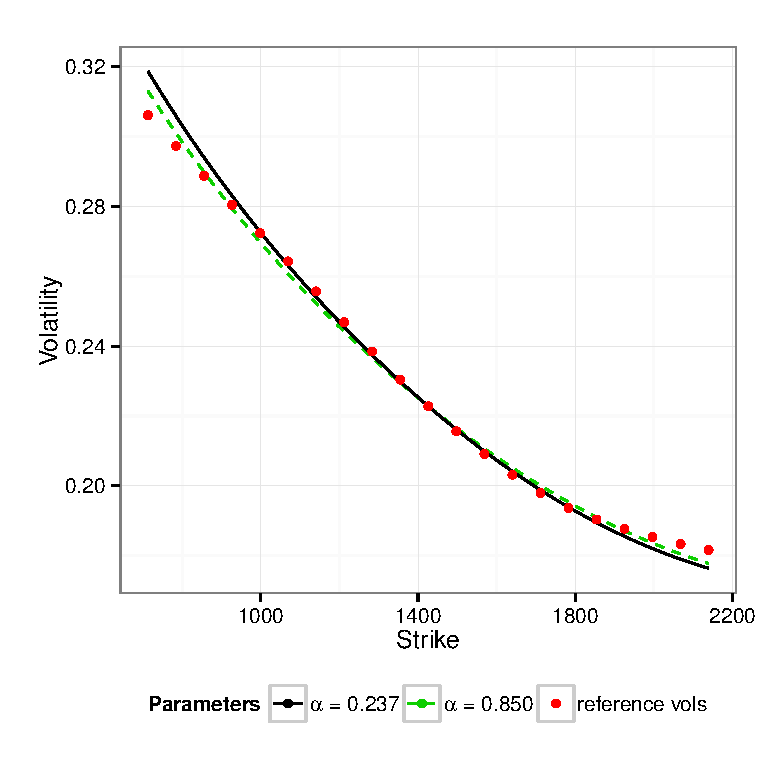
\includegraphics[width=14cm]{two_sabr_1_smile.eps}
\end{center}
\end{figure}
The fact that two different SABR parameters sets can lead to smiles with nearly the same error measure is the root of issues with differential evolution: it is not obvious which set of parameter is the right one without some additional constraint on the variation of the parameters. This can be resolved by some penalty term, but it is difficult in practice to find the correct penalty term that works for a variety of situations. A better approach would be look beyond the best candidate, and consider as alternative initial guesses the other candidates in the latest generation with very similar error measure and different (lower) $\alpha$. In contrast, the explicit guess leads directly to the correct smile.

\subsubsection{Swaption smiles}
We apply the same calibration methodology as for the equity smiles cases, but relying on the normal formula with $\beta=0.5$ instead. The calibrated parameters are indistinguishable between the calibration on the explicit initial guess and the calibration on the guess found by differential evolution (see Table \ref{tbl:normal_sabr_fit}). Furthermore, the initial guess is very close to the calibration result. 

\begin{table}[h]
\begin{center}
\caption{\label{tbl:normal_sabr_fit}calibrated SABR parameters with $\beta=0.5$. LM denotes Levenberg-Marquardt minimization.}
\begin{tabular}{c c c c c c}
\hline
Method & $\alpha$ & $\rho$ &$\nu$ & normal vol RMSE & time(ms) \\
\hline
\multicolumn{6}{c}{1m5y swaption in May 2014, $f=0.0184$}\\
\hline
Explicit & 0.052 & 0.458 & 0.751 & 2.95e-04 & 0.01 \\
Explicit + LM  & 0.052 & 0.368 & 0.768 & 2.39e-04 & 0.11\\
Differential Evolution + LM  & 0.052 & 0.368 & 0.768 & 2.39e-04 & 5.17 \\
\hline
\multicolumn{6}{c}{2y5y swaption in May 2014, $f=0.0309$}\\
\hline
Explicit & 0.052 & 0.060 & 0.322 & 1.43e-05 & 0.01 \\
Explicit + LM & 0.052 & 0.058 & 0.313 & 7.59e-06 & 0.10\\
Differential Evolution + LM & 0.052 & 0.058 & 0.313 & 7.59e-06 & 1.95\\
\hline
\multicolumn{6}{c}{10y10y swaption in May 2014, $f=0.0398$}\\
\hline
Explicit & 0.037 & -0.141 & 0.319 & 2.26e-05 & 0.01 \\
Explicit + LM  & 0.037 & -0.153 & 0.305 & 4.68e-06 & 0.12\\
Differential Evolution + LM  & 0.037 & -0.153 & 0.305 & 4.68e-06 & 3.67\\
\hline
\end{tabular}
\end{center}
\end{table}
Figures \ref{fig:explicit_fit_1m_beta05}, \ref{fig:explicit_fit_2y_beta05} and \ref{fig:explicit_fit_10y_beta05} show how close are the smile produced by the initial guess and the smile resulting from the Levenberg-Marquardt minimization for short expiries as well as for long ones.
\begin{figure}[h!]
  \caption{\label{fig:explicit_fit_1m_beta05}Initial guess and calibrated smile for a May 2014 1m5y Swaption }
\begin{center}
 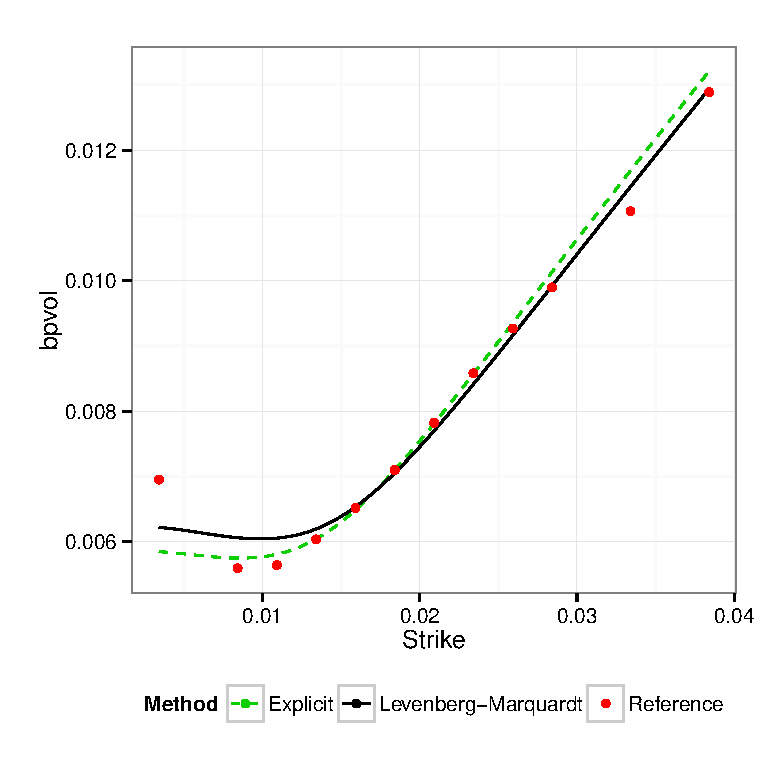
\includegraphics[width=13cm]{explicit_fit_1m_beta05.eps}
\end{center}
\end{figure}

\begin{figure}[htb]
  \begin{center}  
      \subfigure[\label{fig:explicit_fit_2y_beta05}2y5y Swaption]{
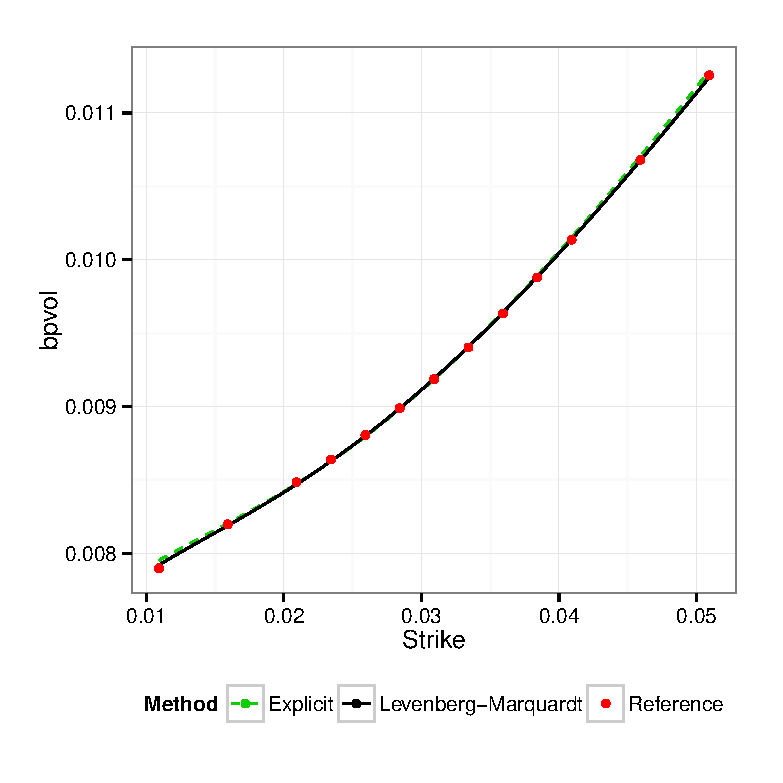
\includegraphics[width=7cm]{explicit_fit_2y_beta05.eps}}
    \subfigure[\label{fig:explicit_fit_10y_beta05}10y10y Swaption]{
  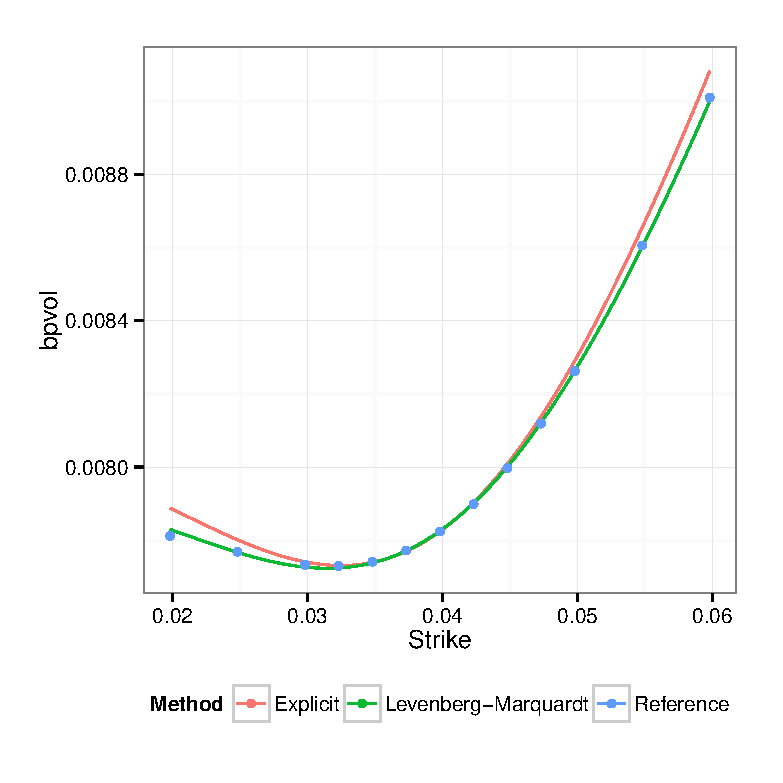
\includegraphics[width=7cm]{explicit_fit_10_beta05.eps} }
  \end{center}
     \caption{Initial guess and calibrated smile}
\end{figure}


\subsection{Calibration on the arbitrage free PDE}
We calibrate the same swaptions as in the previous section but using the arbitrage free SABR model from \citep{hagan2013arbitrage}. In the calibration procedure there is the need to transform the swaption price resulting from integrating the probability density to a normal volatility, in order to compute the error in terms of normal volatilities. This can be achieved with near machine accuracy using the algorithm from \citep{lefloch2014bpvol}. The transformation to normal volatitilies must be reasonably accurate for extremely low option prices, as even if the options reference prices are not so low, the prices resulting from the best fit procedure can be extremely low.

Short and medium expiries calibrated SABR parameters are very close to the one of the previous section (Table \ref{tbl:arbfree_sabr_fit}).
\begin{table}[h]
\begin{center}
\caption{\label{tbl:arbfree_sabr_fit}calibrated SABR parameters with $\beta=0.5$ for the arbitrage free SABR model. LM denotes Levenberg-Marquardt minimization.}
\begin{tabular}{c c c c c c}
\hline
Method & $\alpha$ & $\rho$ &$\nu$ & normal vol RMSE & time(s) \\
\hline
\multicolumn{6}{c}{1m5y swaption in May 2014}\\
\hline
Explicit & 0.052 & 0.458 & 0.751 & 2.87e-04 & 0.005 \\
Explicit+LM & 0.052 & 0.374 & 0.765 & 2.40e-04 & 0.071\\
\hline
\multicolumn{6}{c}{2y5y swaption in May 2014}\\
\hline
Explicit & 0.052 & 0.055 & 0.328 & 1.40e-05 & 0.005\\
Explicit+LM & 0.052 & 0.058 & 0.323 & 6.61e-06 & 0.081\\
\hline
\multicolumn{6}{c}{10y10y swaption in May 2014}\\
\hline
Explicit & 0.037 & -0.145 & 0.322 & 7.36e-05 & 0.005\\
Explicit+LM & 0.037 & -0.194 & 0.359 & 6.97e-06 & 0.068\\
\hline
\end{tabular}
\end{center}
\end{table}

There is however a visible difference for the longest expiry. In particular, the SABR parameters $\rho, \nu$ have a slightly different meaning: the smile resulting from the normal explicit initial guess is lower for low strikes with the arbitrage free PDE approach than the smile computed from the same guess with the normal formula (Figure \ref{fig:normal_vs_arbfree_fit_10y10y}).

\begin{figure}[htbp]
  \caption{\label{fig:normal_vs_arbfree_fit_10y10y}Initial guess and calibrated smile for a May 2014 10y10y Swaption using the Arbitrage-free SABR PDE approach }
\begin{center}
 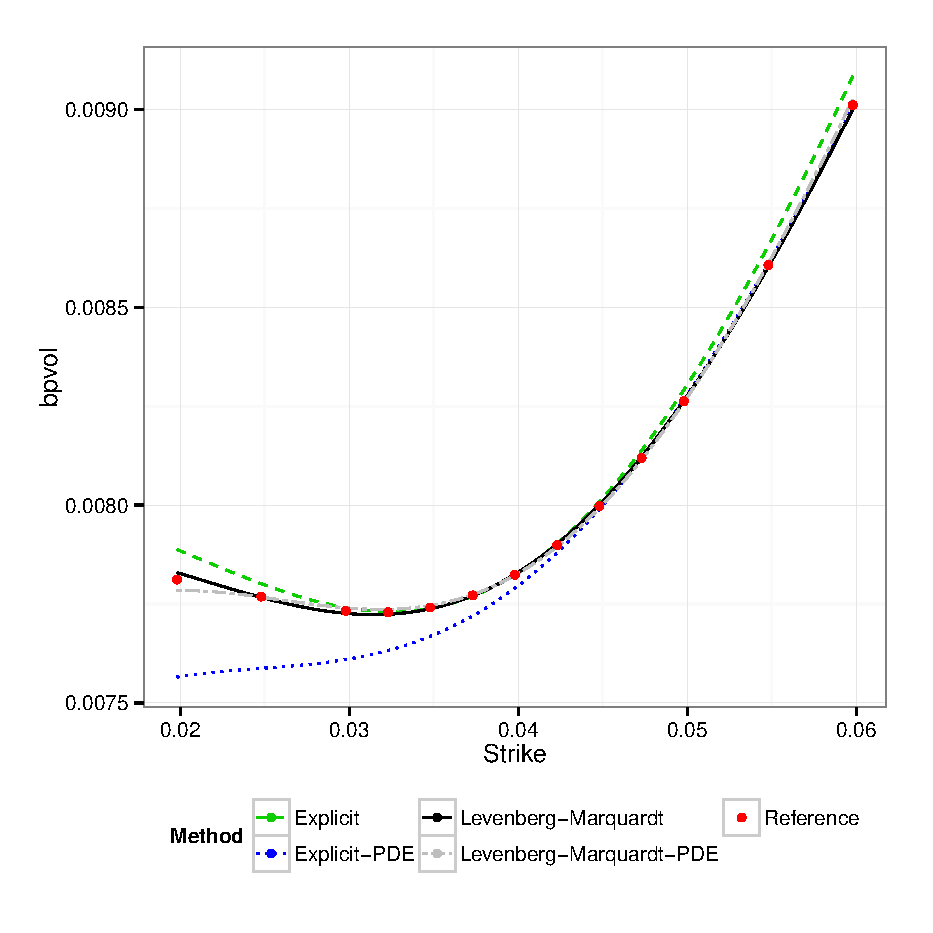
\includegraphics[width=12cm]{normal_vs_arbfree_fit_10y10y.eps}
\end{center}
\end{figure}

\section{Conclusion}
We have presented an explicit initial guess procedure to calibrate the lognormal SABR formula as well as the normal SABR formula, that, despite its simplicity, works particularly well for a variety of different SABR configurations. It allows for faster calibration, by using only a local minimizer, as well as a more reliable calibration, by avoiding the problem of multiple best fits that can appear with global minimizers. 

We have shown it can also be applied to the arbitrage free SABR model with success, even if the guess is further away from the target for longer maturities, due to the mismatch between the arbitrage free SABR model and the classic normal SABR formula.

The same approach to calibration, namely to recover model parameters of a second or third order expansion from a best fit parabola or cubic can be applied to other models. Such expansions can be relatively easily derived for a large class of stochastic (local) volatility models using the techniques of \citep{lorig2014implied}.
\newpage
\appendix
\section{Simple expansion of the normal formula}\label{apx:normal_expansion}
A Taylor expansion of the normal formula (Equation \ref{eqn:normal_sabr}) in $z = \log\frac{K}{f}$ and $\alpha$ leads to:
\begin{align*}
\sigma_N(z, \alpha) &=−\frac{\left( \left( 3\,{f}^{\beta}\,{\nu}^{2}\,{\rho}^{2}−2\,{f}^{\beta}\,{\nu}^{2}\right) \,T-24\,{f}^{\beta}\right) \,\alpha}{24}+\frac{\beta\,{\left( {f}^{\beta}\right) }^{2}\,\nu\,\rho\,T\,{\alpha}^{2}}{4\,f}\\
&-\frac{\left( 3\,f\,{\nu}^{3}\,{\rho}^{3}-2\,f\,{\nu}^{3}\,\rho\right) \,z\,T-24\,f\,\nu\,\rho\,z}{48}\\
&+\frac{\left( \left( 3\,\beta\,{f}^{\beta}\,{\nu}^{2}\,{\rho}^{2}+2\,\beta\,{f}^{\beta}\,{\nu}^{2}\right) \,z\,T+24\,\beta\,{f}^{\beta}\,z\right) \,\alpha}{48}+\frac{\left( 13\,{\beta}^{2}-8\,\beta\right) \,{\left( {f}^{\beta}\right) }^{2}\,\nu\,\rho\,z\,T\,{\alpha}^{2}}{48\,f}\\
&+\frac{\left( 9\,{f}^{2}\,{\nu}^{4}\,{\rho}^{4}-12\,{f}^{2}\,{\nu}^{4}\,{\rho}^{2}+4\,{f}^{2}\,{\nu}^{4}\right) \,{z}^{2}\,T+\left( -72\,{f}^{2}\,{\nu}^{2}\,{\rho}^{2}+48\,{f}^{2}\,{\nu}^{2}\right) \,{z}^{2}}{288\,{f}^{\beta}\,\alpha}
\\&-\frac{\left( \left( 6\,\beta+3\right) \,f\,{\nu}^{3}\,{\rho}^{3}+\left( -4\,\beta-2\right) \,f\,{\nu}^{3}\,\rho\right) \,{z}^{2}\,T-24\,f\,\nu\,\rho\,{z}^{2}}{96}\\
&+\frac{\left( \left( \left( 12\,{\beta}^{2}+3\,\beta\right) \,{f}^{\beta}\,{\nu}^{2}\,{\rho}^{2}+\left( 4\,{\beta}^{2}-2\,\beta\right) \,{f}^{\beta}\,{\nu}^{2}\right) \,{z}^{2}\,T+\left( 24\,{\beta}^{2}+24\,\beta\right) \,{f}^{\beta}\,{z}^{2}\right) \,\alpha}{288}\\
&+\frac{\left( 13\,{\beta}^{3}-15\,{\beta}^{2}+5\,\beta\right) \,{\left( {f}^{\beta}\right) }^{2}\,\nu\,\rho\,{z}^{2}\,T\,{\alpha}^{2}}{96\,f}
 + o(z^2)
 + o(\alpha^2)
\end{align*}
Assuming that $\nu$ is also small and neglecting higher order cross terms leads to our simple expansion.

\section{Least squares parabola}\label{apx:parabola}
The parabola $a + b x + c x^2$ that minimizes the square error $E=\sum_{i=1}^{n} w_i\left(y_i - (a + b x_i + c x_i^2)\right)^2 $ at the points $(x_i, y_i)$ with weights $w_i$ verifies:
\begin{align}
\begin{cases}
\frac{\partial E}{\partial a} &= 2\sum\limits_{i=1}^{n} w_i\left(y_i - (a + b x_i + c x_i^2 )\right) = 0\\
\frac{\partial E}{\partial b} &= 2\sum\limits_{i=1}^{n} w_i x_i \left(y_i - (a + b x_i + c x_i^2 )\right) = 0\\
\frac{\partial E}{\partial c} &= 2\sum\limits_{i=1}^{n} w_i x_i^2 \left(y_i - (a + b x_i + c x_i^2 )\right) = 0
\end{cases}
\end{align}
The coefficients $a, b, c$ are the solution of the following linear system:
\newcommand{\FF}{\vphantom{\sum\limits_{i=1}^{n}}}
\begin{equation}
\begin{pmatrix}
\sum\limits_{i=1}^{n} w_i & \sum\limits_{i=1}^{n} w_i x_i & \sum\limits_{i=1}^{n} w_i x_i^2 \\
\sum\limits_{i=1}^{n} w_i x_i & \sum\limits_{i=1}^{n} w_i x_i^2 & \sum\limits_{i=1}^{n} w_i x_i^3 \\
\sum\limits_{i=1}^{n} w_i x_i^2 & \sum\limits_{i=1}^{n} w_i x_i^3 & \sum\limits_{i=1}^{n} w_i x_i^4  
\end{pmatrix}
\begin{pmatrix}
\FF a\\
\FF b\\
\FF c
\end{pmatrix}
=
\begin{pmatrix}
\sum\limits_{i=1}^{n} w_i y_i\\
\sum\limits_{i=1}^{n} w_i x_i y_i\\
\sum\limits_{i=1}^{n} w_i x_i^2 y_i
\end{pmatrix}
\end{equation}
It can be useful to pin a specific point $(f,\sigma_f)$, for example to make sure that the at-the-money volatility is exactly represented by the parabola as it is available in the swaption market. In this case the system to solve becomes:
\begin{equation}
\begin{pmatrix}
\FF 1 & f & f^2 \\
\sum\limits_{i=1}^{n} w_i x_i & \sum\limits_{i=1}^{n} w_i x_i^2 & \sum\limits_{i=1}^{n} w_i x_i^3 \\
\sum\limits_{i=1}^{n} w_i x_i^2 & \sum\limits_{i=1}^{n} w_i x_i^3 & \sum\limits_{i=1}^{n} w_i x_i^4  
\end{pmatrix}
\begin{pmatrix}
\FF a\\
\FF b\\
\FF c
\end{pmatrix}
=
\begin{pmatrix}
\FF \sigma_f\\
\sum\limits_{i=1}^{n} w_i x_i y_i\\
\sum\limits_{i=1}^{n} w_i x_i^2 y_i
\end{pmatrix}
\end{equation}
\bibliographystyle{rAMF}
%\bibliographystyle{ieeetr}
\bibliography{lefloch_smart_sabr}


\end{document}
